\chapter{Proposed system}\label{ch:model}
This chapter first discusses BGP behavior and its implications on a hijack detection scheme. Including in this section, a new type of hijack is explained. Then, available information sources are discussed, after which the actual detection algorithm will be described. This model will be referred to as the BGP Hijack Alert System (BHAS).

\section{Design considerations}\label{sec:sourcesofinformation}
At this moment (January 26th 2016), the full BGP table counts a total number of 616.022 announced IPv4\cite{ipv4report} and IPv6\cite{ipv6report} prefixes. Back in 2005, an average of 1600 BGP updates were sent over the Default Free Zone (DFZ) every hour\cite{huston2006projecting}. Routers in the DFZ have no default route, e.g. null route configured\cite{berkowitz2005terminology}. In terms of routing information they are entirely dependent of routes received from their neighbors. Studies predicted a significant growth towards 2.8 million updates per hour at the end of 2010\cite{huston2006projecting}.\par
Figure \ref{fig:ipv4prefixes} and \ref{fig:ipv6prefixes} illustrate the continuing trend of the increasing size of the BGP Forward Information Base (FIB) of routers in the DFZ. This table is used by routers when forwarding traffic\cite{berkowitz2005terminology}. Hijack detection systems working with control-plane data need to be able to process this information near real-time.\\\par
\begin{figure}[hb!]
\RawFloats
\centering
\begin{minipage}{.5\textwidth}
  \centering
  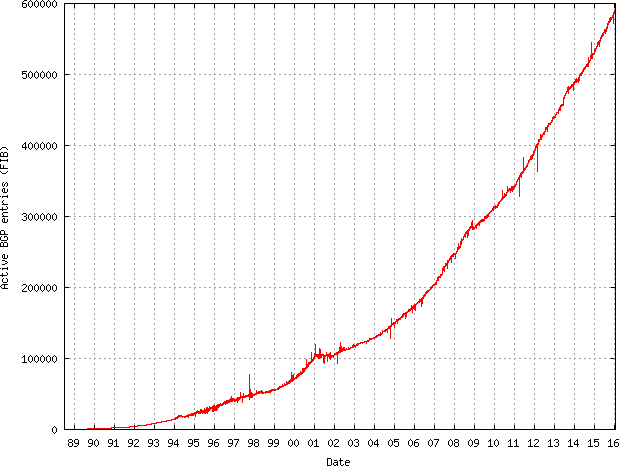
\includegraphics[scale=0.32]{images/plot-ipv4.png}
  \caption{The growth of IPv4 prefixes \cite{plotipv4}}
  \label{fig:ipv4prefixes}
\end{minipage}%
\begin{minipage}{.5\textwidth}
  \centering
  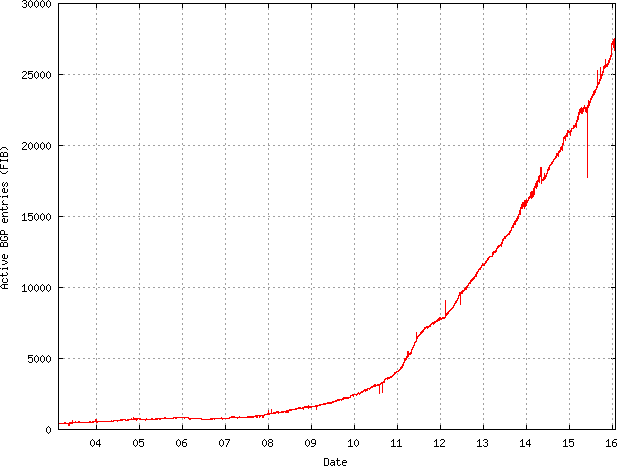
\includegraphics[scale=0.32]{images/plot-ipv6.png}
  \caption{The growth of IPv6 prefixes \cite{plotipv6}}
  \label{fig:ipv6prefixes}
\end{minipage}
\end{figure}

\subsection{BGP hijack types}\label{subsec:modelbgphijacktypes}
The four types of hijacks specified in section \ref{sec:hijacks} will categorize many hijacks. However, another type of hijack was worked out during this research. This is called a less specific, or a supernet hijack (later referenced to as a type 5 hijack). Briefly, a less specific hijack can be described as an announcement of a large IP prefix which itself is not being announced, but has more specific prefixes that are. This leverages the route to spread over the internet. For most network blocks below this route, i.e. networks sharing the network part, but with a higher subnet mask, there will be a more specific route known. These networks won't be affected, as BGP's routing decisions prefer more specific routes\cite{rekhter2006rfc}. However, depending on the hijacked prefix, there might be an address block which is not yet being explicitly advertised. This IP space within the hijacked prefix will be routed to the malicious router advertising the less specific prefix. Especially unused prefixes are vulnerable for a less specific hijack. The proposed model is capable of detecting all five types of hijacks. In table \ref{table:hijacktypes} all five hijack types are summarized, including their ID which will be referred to later in this paper.\par

\begin{table}[h]
        \centering
        \begin{tabular}{p{0.5cm}|p{4cm}|p{4cm}|p{4cm}|}
                \textbf{\#} & \textbf{Name} & \textbf{Announcing AS} & \textbf{Annnounced Prefix} \\ \hline
                1 & Prefix hijack\cite{hu2007accurate} & $\neq$ authorized AS & = monitored prefix \\ \hline
                2 & Subnet hijack\cite{hu2007accurate} & $\neq$ authorized AS & $\subset$ monitored prefix \\ \hline
                3 & Prefix \& AS hijack\cite{hu2007accurate} & = authorized AS & = monitored prefix \\ \hline
                4 & Subnet \& AS hijack\cite{hu2007accurate} & = authorized AS & $\subset$ monitored prefix \\ \hline
                5 & Supernet hijack & $\neq \lor$ = authorized AS & $\supset$ monitored prefix \\ \hline
        \end{tabular}
        \caption{Comparison of all hijack types}
        \label{table:hijacktypes}
\end{table}

\subsection{Utilized information sources}\label{subsec:utilizedinformationsources}
This section describes all sources of information that will be used for detecting BGP hijacks.

\paragraph{BGP feed}\label{par:ripestat}\mbox{ }\\
In order to detect prefix hijacks as soon as possible, BGP UPDATE messages are collected from a full BGP feed sent by the core routers of an ISP. A full BGP feed contains a stream of updates from all public AS numbers all over the world. Private AS number updates are not re-advertised by an ISP, these are advertised by an aggregated prefix from the ISP. BGP updates contain, amongst others, an AS path which is displayed in equation figure \ref{eq:aspath}. This is the path of Autonomous Systems to traverse from a neighbor peer to the destination AS where the prefix resides. This paper later refers to two elements in the AS path, namely the origin AS and the upstream AS. The origin AS is $AS_{N}$, whereas the upstream AS is the second last AS in the AS path, namely ($AS_{N-1}$).

\begin{equation}
\label{eq:aspath}
U_{as\_path} = \{ AS_{0}, AS_{1}, \ldots, AS_{N-1}, AS_{N} \}
\end{equation}

%This project assumes that hijacks within the domain of an ISP will not happen or will not be announced by the ISP. Therefore these hijacks will not be noticed by the model.

\paragraph{RIPEstat API}\label{par:ripestat}\mbox{}\\
Metadata regarding Autonomous Systems and BGP prefixes are collected through the RIPEstat API\cite{ripestats}. This API (Application Programmable Interface) is maintained by RIPE, the Regional Internet Registry (RIR) of Europe. Its sources of information includes authority data of other RIR's and geographical information of MaxMind\cite{maxmindgeoip}. RIPEstat is used to retrieve the correct AS numbers and country codes for every monitored prefix. These AS numbers originate from the Internet Routing Registry (IRR), and represent the Autonomous Systems that are allowed to announce a certain prefix, also known as routing policies\cite{battista2006extractbgp}. As to be seen in table \ref{table:ripestaturis}, this data shall be of great value when detecting various hijack types. Details regarding the IRR itself will be discussed in the next paragraph.\par

\begin{table}[h]
        \centering
        \begin{tabular}{|p{2cm}|p{4cm}|p{5cm}|}\hline
                \textbf{Resource} & \textbf{Utilized for} & \textbf{Description}  \\ \hline
                geoloc & BHAS & Determine geolocation of monitored prefix origin AS \\ \hline
                geoloc & BHAS & Determine geolocation of BGP update upstream AS \\ \hline
%                geoloc & Compare geolocation of update upstream AS to origin AS & 3, 4 \\ \hline
                whois & BHAS & IRR records, obtain authorized ASNs for prefix \\ \hline
                whois & Research IRR coverage & IRR records, obtain authorized ASNs for prefix \\ \hline
                announced-prefixes & Research IRR coverage & Obtaining currently announced prefixes for a given AS \\ \hline
        \end{tabular}
        \caption{Utilized resources from RIPEstat API}
        \label{table:ripestaturis}
\end{table}

When querying the RIPEstat API, prefix information is disclosed to RIPE. However, RIPE allows the database to be downloaded. RIPE offers a daily snapshot of the database, in which personal contact information has been omitted, available for download from an FTP mirror\cite{downloadripedb}. Another option is to anonymize requests through the use of Tor or a Virtual Private Network (VPN).

\paragraph{Internet Routing Registry (IRR)}\label{par:irr}\mbox{}\\
As mentioned in paragraph \ref{par:ripestat}, the IRR contains a set of routing policies which is maintained by participating organizations, for example, prefix owners. This model will use the IRR to detect legitimate MOAS conflicts. According to performed research\cite{routehygiene, irraccuracy, battista2006extractbgp}, the IRR is not complete at all. As this research was published in 2009 and earlier, the current coverage of all Dutch ASes in the IRR need to be researched in order to determine whether the IRR is a usable resource. The strategy for doing so will be discussed in the next paragraph.
\newpage
\paragraph{CIDR report}\mbox{}\\
In order to retrieve a list with all Dutch Autonomous System Numbers, CIDR Report was used. This websites publishes, amongst others a list of issued AS numbers, including per AS country code of the issued party\cite{huston2005cidr}.

\subsection{Excluded information sources}\label{subsec:excludedsources}
This section explains why certain public resources were not used for this project.

\paragraph{Looking glasses}\label{par:lookingglasses}\mbox{}\\
Looking glasses can provide valuable information. However, it conflicts with the requirement not to leak any private information, like prefixes or AS numbers to third parties. Therefore, the decision was taken not to use them as a source of information for detecting prefix hijacks. However, as almost 200 looking glass server worldwide are open for querying, it is interesting future work to add this information source\cite{zhang2005collecting}.

\paragraph{RouteViews}\label{par:routeviews}\mbox{}\\
The University of Oregon publishes BGP announcement data, collected from several locations over the world. Although this data is approximately two hours behind in time\cite{routeviews}, collecting BGP updates from multiple vantage points worldwide can be of great value. These incremental BGP Update messages are MRT\cite{rfc6396} formatted and can be collected from an FTP mirror. Since BGP routers only advertise their most preferred route to a destination, a single BGP feed will give a limited view. Utilizing feeds from geographically distant vantage points is advised to improve the near real-time detection of hijacks\cite{zhang2007impact}. As a full BGP feed has already been setup for this project, RouteViews will not be used. For now, it is considered as future work. \par 

\section{Architecture}\label{sec:architecture}
This chapter discusses the architecture of the BGP Hijack Alert System. In figure \ref{fig:bhasarchitecture}, the application's architecture can be seen, which will be elaborated on in the upcomping sections. First, the bottom layer will be discussed as this contains elements which will be referred to in the upper layers.

\begin{figure}[hb!]
\RawFloats
\centering
\begin{minipage}{.5\textwidth}
    \centering
    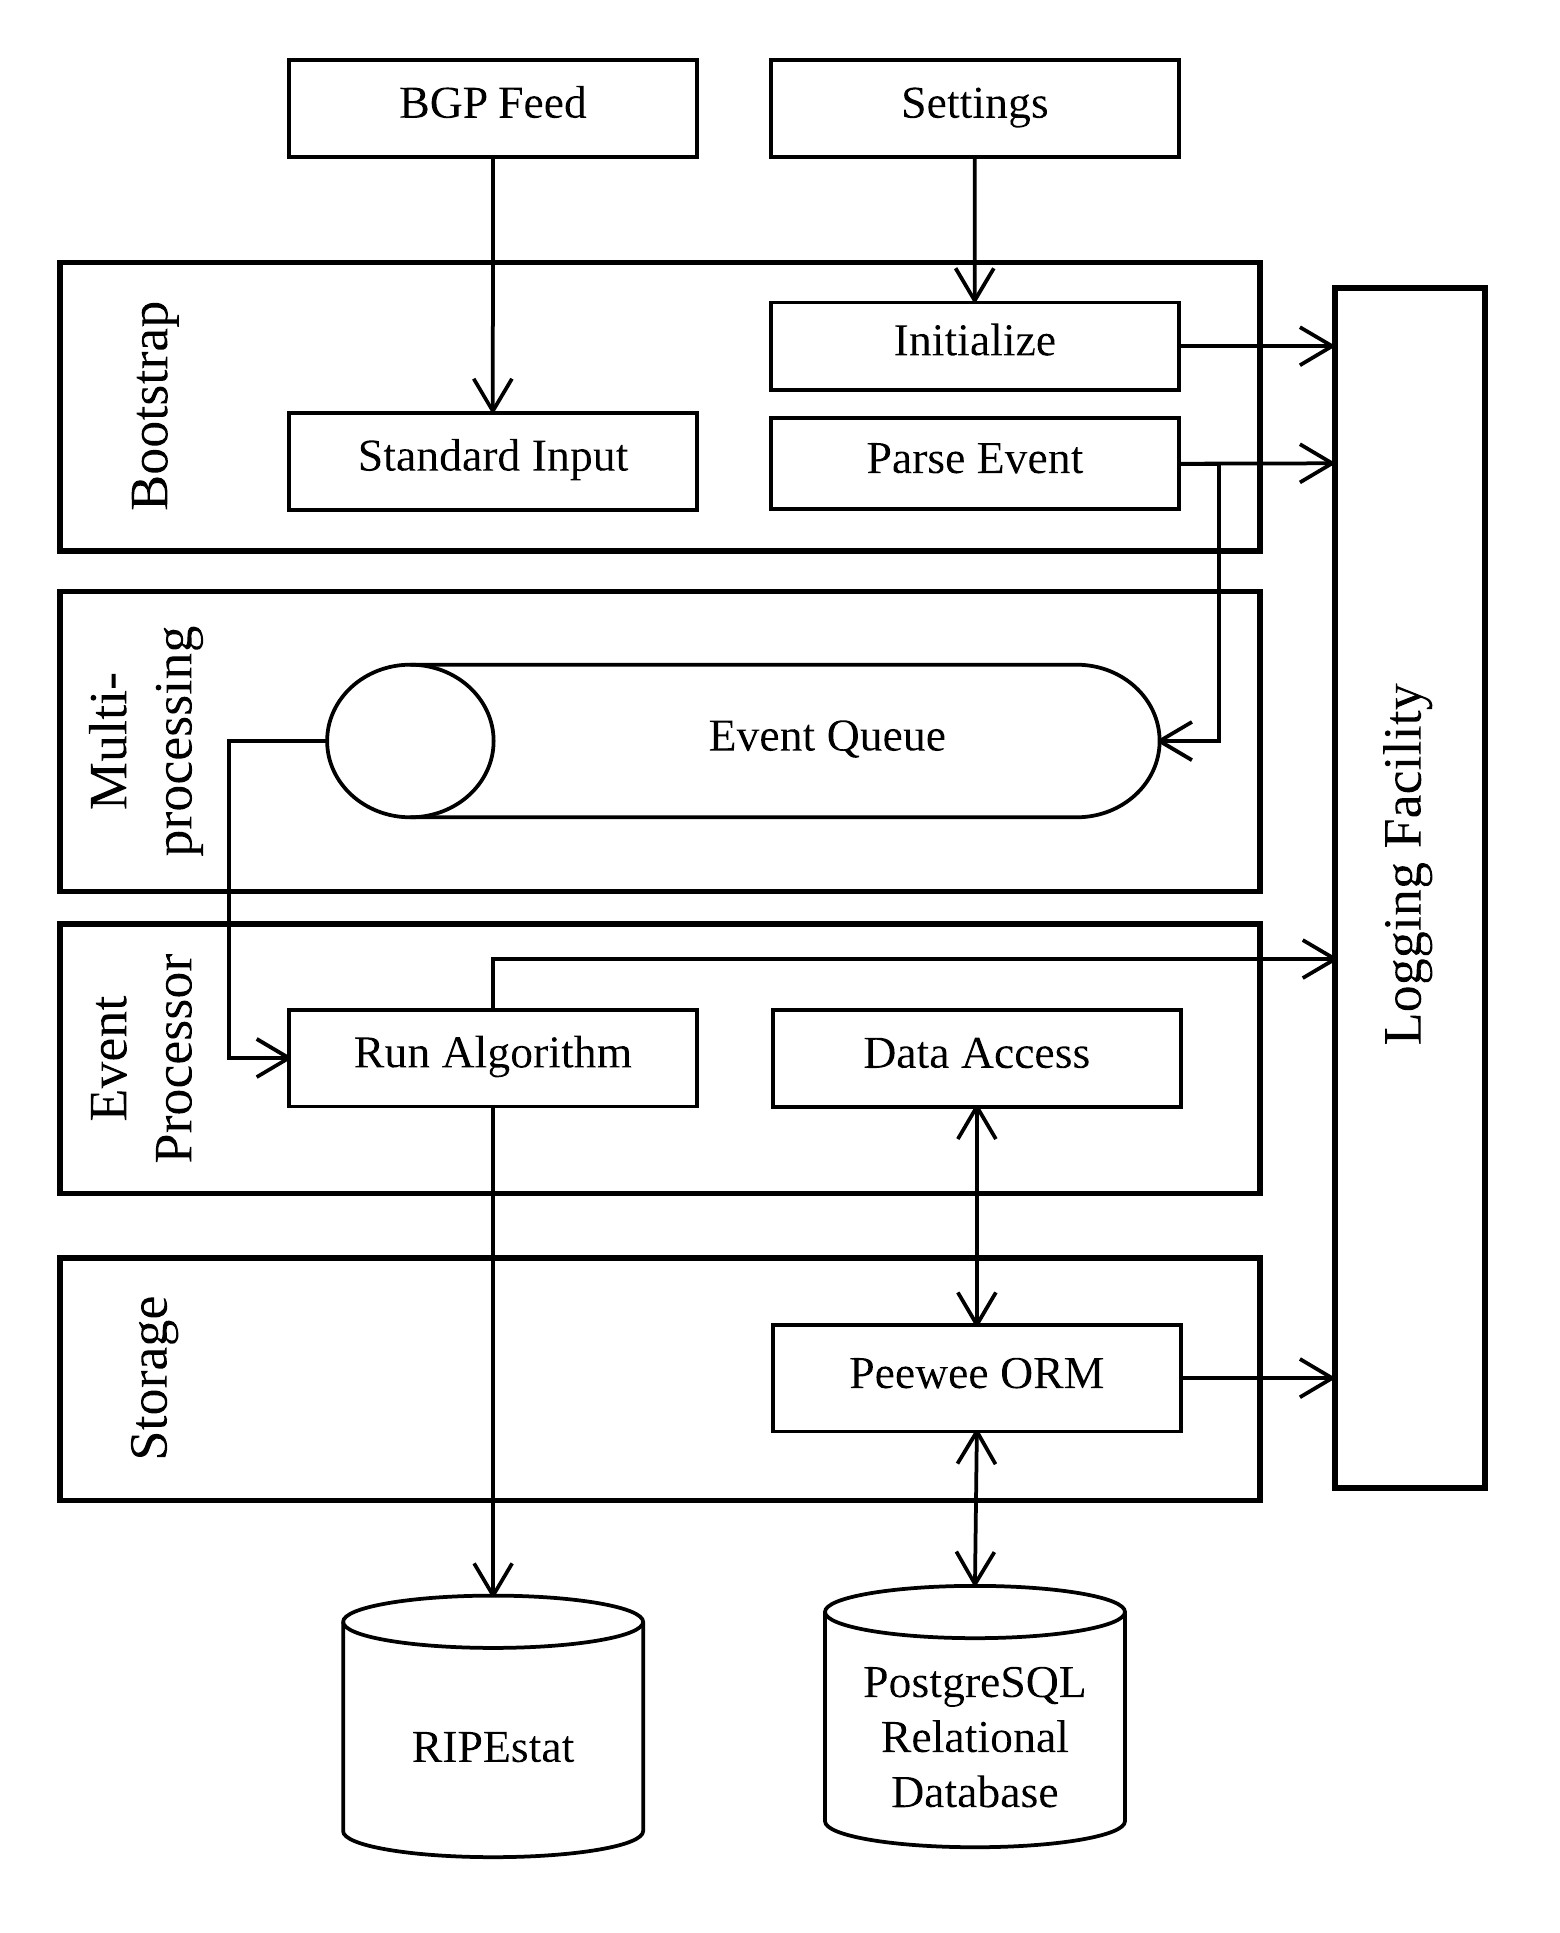
\includegraphics[scale=0.13]{images/architecture.png}
    \caption{BHAS Architecture}
    \label{fig:bhasarchitecture}
\end{minipage}%
\begin{minipage}{.5\textwidth}
    \centering
    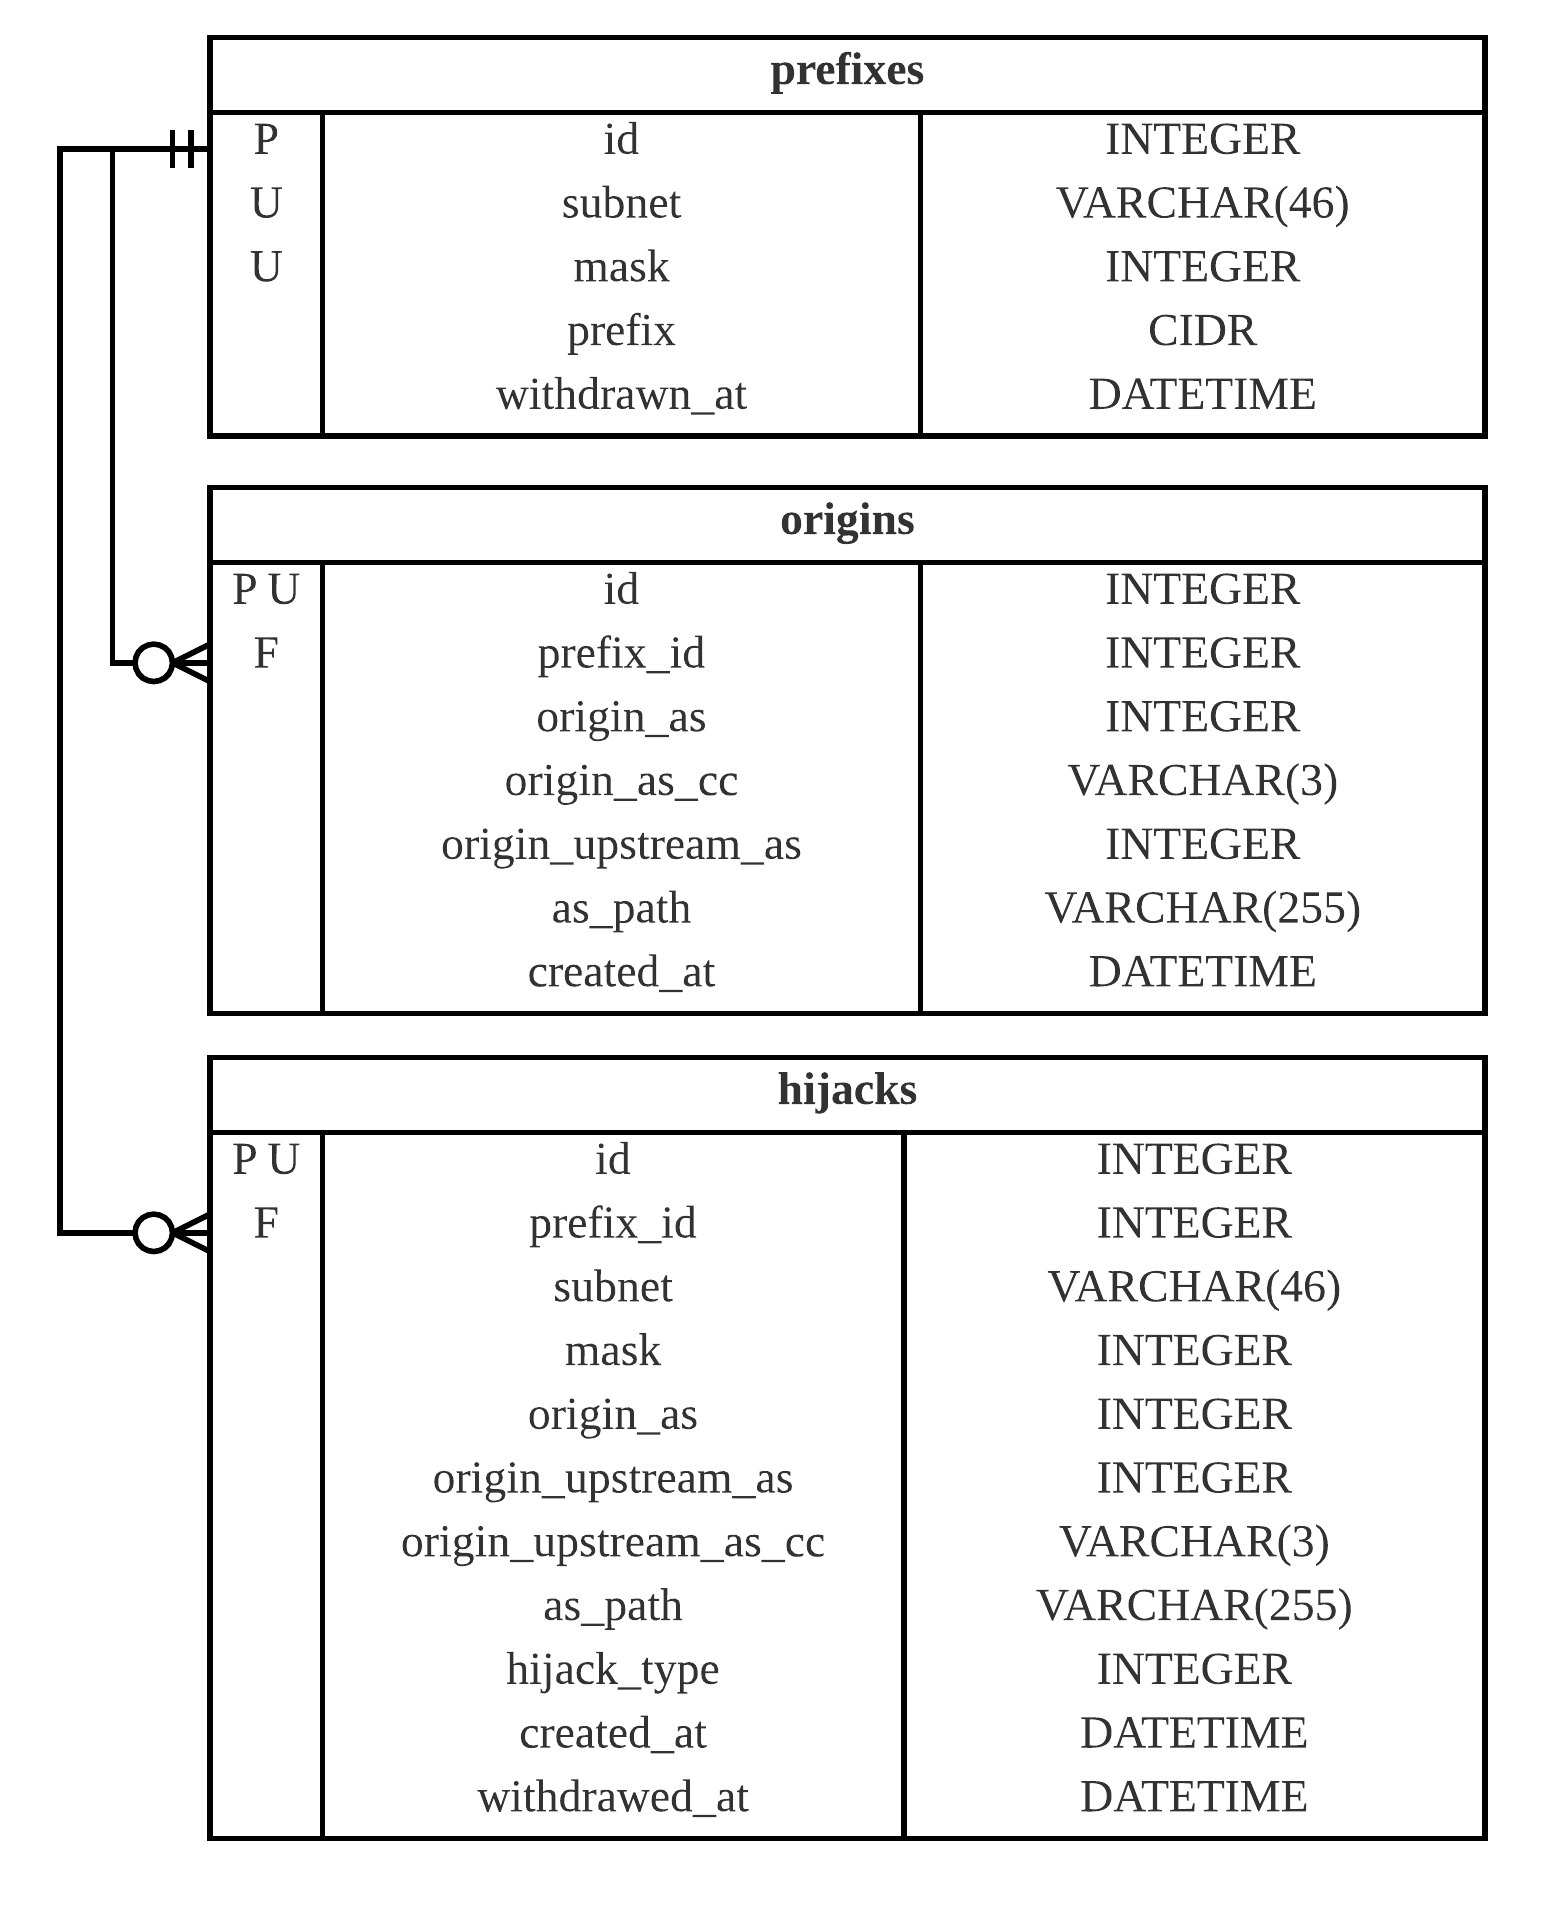
\includegraphics[scale=0.14]{images/erd.png}
    \caption{BHAS Entity Relationship Diagram (ERD)}
    \label{fig:erddatabase}
\end{minipage}
\end{figure}

\subsection{Software router}\label{subsec:softwarerouter}
In order to process the BGP feed a low level entry point into a routers software is required. No vendor will provide this kind of entry point to the source code of a router. Therefore a software router must be used to make this model work. Some different software routers are available. Quagga\cite{quagga}, EXAbgp\cite{exabgp} and BIRD \cite{bird} are compared. Quagga is easy to use because of the Cisco like command line interface (cli) but its it harder to create an output for BGP updates. EXAbgp on the other hand is harder to configure and has its own set of commands but the way it outputs received information is very easy to use and control. BIRD is the last product compared in table \ref{table:softwarerouter}. BIRD is not able to produce useful output for further analysis. BHAS uses EXAbgp to receive the BGP feed and feeds it to the algorithm. 

\par

\begin{table}[]
\centering
\begin{tabular}{|l|l|l|l|}
    \hline
    \textbf{Feature}                   & \textbf{EXAbgp}\cite{exabgp}  & \textbf{BIRD}\cite{bird} & \textbf{Quagga}\cite{quagga} \\ \hline
    CLI                                & None             & None                      & Cisco CLI       \\ \hline
    Output formats                     & JSON, plain text & None                      & MRT             \\ \hline
    Support program execution          & Yes              & No                        & No              \\ \hline
    Runtime change                     & No               & Yes                       & Yes             \\ \hline
    Protocol support                   & BGP              & BGP, RIP, OSPF, \ldots    & BGP, RIP, OSPF, \ldots             \\ \hline
\end{tabular}
\caption{Software router comparison}
\label{table:softwarerouter}
\end{table}

\subsection{Storage}\label{subsec:bhasstorage}
BHAS uses Object Relational Mapping (ORM) to map application objects to database entities. Regarding database storage, three tables are used to respectively store the monitored prefixes, their origins and observed hijacks. In figure \ref{fig:erddatabase}, the Entity Relationship Diagram displays these database entities and their properties. A monitored prefix uses a CIDR datatype which is only available in PostgreSQL and allows the database engine to compare prefixes\cite{postgresqlcidr}. Furthermore, a prefix is related to zero or more origins. An origin represents an Autonomous System authorized to announce a prefix, which must always be related to exactly one prefix. A prefix might have no origin at all, when this prefix should not be announced by any AS at all.\par
Alike origins, a hijack should also be linked to exactly one prefix. For every hijack, the AS announcing the sub-or-supernet of the monitored prefix are saved, as well as the upstream AS and its country code, and the complete AS path. The hijack type relates to the five types discussed in section \ref{subsec:modelbgphijacktypes}.

\subsection{Initialization}\label{subsec:bhasinitialization}
As BHAS only monitors a fixed number of prefixes, its database needs to be initialized before the application can start monitoring. A textfile containing a newline seperated list with prefixes in CIDR notation is expected as input. The system will then query all IRR records for every prefix, as well as every prefix's country code and save the result into the database. Per prefix, a new Origin is created for every AS found in the IRR records. The AS Path will be left blank, as it can only be determined upon receiving a BGP announcement originating from this origin.

\subsection{Bootstrap}\label{subsec:bhasbootstrap}
When starting BHAS, the bootstrap component will wait for JSON formatted standard input. The JSON output format of ExaBGP is used as input format for this model. The bootstrapper will try to parse the input into a temporary Event object. It will do so for every prefix encountered in an update message. If successful, the Event is put onto a queue described in the next section. The result of the parsing is written to the logging facility, irrespective of whether the attempt failed or succeeded.

\subsection{Multiprocessing}\label{subsec:bhasmultiprocessing}
The main program of BHAS utilizes two processes, sharing a queue. While one process converts \emph{stdin} to Event objects which it places on the queue, the second process which is described in the next paragraph runs the algorithm for every object on the queue. Since the order of the queue objects matters, the decision was made not to use multiple processes simultaneously processing the queue. Hence, only two processes exists. Still, multiprocessing enables the program to process the input fast, without having to wait for the bottom layers to complete API calls or database access.

\subsection{Event processor}\label{subsec:bhaseventprocessor}
Together with the Bootstrap, this is BHAS its main component. The event processor pulls Event objects off the queue in a FIFO (First-In First-Out) manner. These objects are then fed to the algorithm, which will be described in section \ref{sec:algorithm}. At this point, the database may be accessed and HTTP calls are performed to the RIPEstat API. The result of the algorithm is written to the logging facility in order to ease debugging. Depending on the logging settings, intermediate results may be logged as wel.
\begin{table}[h]
        \centering
        \begin{tabular}{|p{2cm}|p{12cm}|}\hline
                \textbf{Attribute} & \textbf{Description} \\ \hline
                prefix & The announced network noted in CIDR format. \\ \hline
                originAS & This is the AS which is announcing the prefix in the received update. \\ \hline
                ASPath & The complete AS path included in the update, see equation \ref{eq:aspath}. \\ \hline
                upstreamAS & This is $ASPath_{N-1}$. \\ \hline
        \end{tabular}
        \caption{Event object properties}
        \label{table:bhasevent}
\end{table}

\section{Algorithm}\label{sec:algorithm}
In this section, the algorithm function in the Event Processor component is reviewed, see figure \ref{fig:bhasarchitecture}. The BHAS algorithm can be seen as a flowchart in appendix \ref{appendix:flowchart}, and the pseudocode is displayed within this chapter, in algorithm \ref{alg:bhas}.

As explained in the previous section, every prefix in a BGP update is parsed to an Event object. Eventually, this object will be fed to the algorithm. As an Event is a temporary object, it is not mentioned in the ERD, figure \ref{fig:erddatabase}. Therefore, all Event object properties relevant to the algorithm are described in table \ref{table:bhasevent}.

Upon entering the algorithm, the prefix is tested on checked whether it is a subnet, an exact match or a supernet of a network of interest set of prefixes. This set is denoted as P. When no matches are found, the update will be discarded. When it does match with an entry in $P$, BHAS checks whether the update is an announcement or a withdrawal. 

\begin{algorithm}[h]
\begin{algorithmic}[1]
\Procedure{Process prefix update}{update $u$}
\If{$\exists p \in P \mid (p_{prefix} \supseteq u_{prefix}) \lor (p_{prefix} \subseteq u_{prefix})$}
    \State $p \gets (p \in P \mid (p_{prefix} \supseteq u_{prefix}) \lor (p_{prefix} \subseteq u_{prefix}))$
    \If{$u_{type} =$ announcement}
        \If{$\exists o \in O \mid (o_{AS} = u_{originAS}) \land (o_{prefix} = p) $}
            \State $o \gets (o \in O \mid (o_{AS} = u_{originAS}) \land (o_{prefix} = p))$
            \If{$u_{ASPath} \neq o_{ASPath}$}
                \If{$u_{upstreamAS} = p_{upstreamAS}$}
                    \State checkIfHijacked($p$)
                \Else
                    \State $g \gets$ getGeolocation($u_{upstreamAS})$
                    \If{$g = o_{geolocation}$}{ checkIfHijacked($p$) }
                    \Else { hijackAlert($p$, $u$) }
                    \EndIf
                \EndIf
            \Else { checkIfHijacked($p$) }
            \EndIf
        \Else
            \State $R \gets $ getLatestIRR($p$)
            \If{$\exists r \in R \mid r_{originAS} = u_{originAS}$}{ updateDb($p$, $r$) }
            \Else { hijackAlert($p$, $u$) }
            \EndIf
        \EndIf
    \ElsIf{$u_{type} =$ withdrawal}
        \If{$\exists h \in H \mid (h_{prefix} = p) \land (\neg h_{withdrawnAt})$}{ clearHijack($p$) }
        \Else{ withdrawPrefix($p$) }
        \EndIf
    \EndIf
\Else{ discard($u$) }
\EndIf
\EndProcedure
\Function{checkIfHijacked}{prefix $p$}
\If{$\exists h \in H \mid (h_{prefix} = p) \land (\neg h_{withdrawnAt})$}{ clearHijack($p$) }
\Else{ discard($u$) }
\EndIf
\EndFunction
\end{algorithmic}
\caption{Hijack Detection Algorithm}
\label{alg:bhas}
\end{algorithm}

\paragraph{Announcements}\label{par:announcements}\mbox{}\\
If the update is an announcement, an origin is searched such that the origin is related to $p$, and the origin's AS matches the announcement's AS. If so, the origin is considered equal.\par
Whenever no matching origin is found, it might be the case that the monitored prefix has been transferred to another Autonomous System. In order to verify, the prefix its latest IRR records are queried from RIPEstat. If an origin in the IRR records is tested equal to an origin in $p_{origins}$, the origin is added to the database. If not, a hijack alert is raised. Depending on the announced prefix to be a sub-or-superset of the monitored prefix, the hijack will be either of type one, two or five.\par

If a matching origin, $o$, was found, the AS path of $o$ is compared to the AS path advertised with the update $u$. If these values correspond, the announcement is considered to originate from the authorized origin. As announcements are only propagated on receiving a better path to a destination, or when the preferred path has been invalidated, the announcement might be caused by a canceled hijack. Therefore, the checkHijack function is initiated (see paragraph \ref{par:checkhijack}).\par

In case the AS path of the origin $o$ and update $u$ did not correspond, a legitimate AS is announcing a monitored prefix from an upstream provider that has never been observed doing so. This might be a legitimate MOAS conflict, for example, when multihoming, caused by a fallback to a secondary ISP. In this case, BHAS assumes the upstream provider should have at least one prefix registered in the same country as the origin AS originates. To perform this check, geolocation data of $u_{upstreamAS}$ is downloaded from the RIPEstat API. If the geolocation data does not match, an AS hijack alert of type three or four is raised.

\paragraph{Withdrawals}\label{par:withdrawals}\mbox{}\\
If the update is checked as a subnet, exact match or a supernet and is recognized as a withdrawal, BHAS will check if a hijack $h$ exists in the set of hijacks $H$ where the hijack is related to $p$. If so, these sub-or-supernet hijacks will be set as withdrawn. When no hijacks are found, the prefix will be checked as withdrawn, but not removed from the set of monitored prefixes. This way, future announcements for this prefix will still be processed by BHAS.

\paragraph{Check hijack}\label{par:checkhijack}\mbox{}\\
This routine is entered whenever an the announcing AS of an update matches a monitored prefix its origin AS, but no further suspicious activity was observed. Therefore, the update is considered to be legitimate. It might be that an attacker has withdrawn a hijack. To verify this, the set of hijacks is checked if there exists a non-withdrawn hijack $h$ related to $p$. If this statement is evaluated to be true, these hijacks are marked as withdrawn. If not, the update is discarded.


